% ============================================================
% Question Bank: ch02-05 Tips, Commissions, and Fees
% Topic Title: Tips, Commissions, and Fees
% CCSS: 7.RP.A.3
% Questions: 30 (18 MC + 7 SA + 5 Graphical)
% ============================================================

% --- Multiple Choice Questions (18) ---

\begin{practiceQuestion}{2-5-q01}{mc}
\begin{questionText}
A restaurant bill is $\$40$. You leave a $15\%$ tip. How much is the tip?
\end{questionText}
\choiceA{$\$4.00$}
\choiceB{$\$5.00$}
\choiceC{$\$6.00$}
\choiceD{$\$8.00$}
\correctAnswer{C}
\explanation{$15\% = 0.15$. Tip: $40 \times 0.15 = \$6.00$.}
\end{practiceQuestion}

\begin{practiceQuestion}{2-5-q02}{mc}
\begin{questionText}
A salesperson earns $8\%$ commission. He sold $\$3{,}000$ worth of furniture. What is his commission?
\end{questionText}
\choiceA{$\$24$}
\choiceB{$\$80$}
\choiceC{$\$240$}
\choiceD{$\$2{,}400$}
\correctAnswer{C}
\explanation{Commission: $3{,}000 \times 0.08 = \$240$.}
\end{practiceQuestion}

\begin{practiceQuestion}{2-5-q03}{mc}
\begin{questionText}
A concert ticket costs $\$65$. There is a $15\%$ service fee. What is the total?
\end{questionText}
\choiceA{$\$9.75$}
\choiceB{$\$55.25$}
\choiceC{$\$74.75$}
\choiceD{$\$80.00$}
\correctAnswer{C}
\explanation{$65 \times 1.15 = \$74.75$.}
\end{practiceQuestion}

\begin{practiceQuestion}{2-5-q04}{mc}
\begin{questionText}
Your dinner bill is $\$52$. You want to leave a $20\%$ tip. Using the $10\%$ shortcut, what is the tip?
\end{questionText}
\choiceA{$\$5.20$}
\choiceB{$\$7.80$}
\choiceC{$\$10.40$}
\choiceD{$\$15.60$}
\correctAnswer{C}
\explanation{$10\%$ of $\$52$ is $\$5.20$. Double it for $20\%$: $5.20 \times 2 = \$10.40$.}
\end{practiceQuestion}

\begin{practiceQuestion}{2-5-q05}{mc}
\begin{questionText}
A real estate agent earns $3\%$ commission on a $\$250{,}000$ home sale. What does she earn?
\end{questionText}
\choiceA{$\$750$}
\choiceB{$\$2{,}500$}
\choiceC{$\$7{,}500$}
\choiceD{$\$75{,}000$}
\correctAnswer{C}
\explanation{$250{,}000 \times 0.03 = \$7{,}500$.}
\end{practiceQuestion}

\begin{practiceQuestion}{2-5-q06}{mc}
\begin{questionText}
A taxi ride costs $\$18$. You tip the driver $18\%$. What is the total you pay?
\end{questionText}
\choiceA{$\$3.24$}
\choiceB{$\$19.80$}
\choiceC{$\$21.24$}
\choiceD{$\$21.60$}
\correctAnswer{C}
\explanation{Tip: $18 \times 0.18 = \$3.24$. Total: $18 + 3.24 = \$21.24$.}
\end{practiceQuestion}

\begin{practiceQuestion}{2-5-q07}{mc}
\begin{questionText}
Mia earns a $5\%$ commission on all sales. She wants to earn $\$500$ this week. How much does she need to sell?
\end{questionText}
\choiceA{$\$2{,}500$}
\choiceB{$\$5{,}000$}
\choiceC{$\$10{,}000$}
\choiceD{$\$25{,}000$}
\correctAnswer{C}
\explanation{$500 \div 0.05 = \$10{,}000$.}
\end{practiceQuestion}

\begin{practiceQuestion}{2-5-q08}{mc}
\begin{questionText}
A website charges a $2.5\%$ transaction fee on every purchase. If you buy something for $\$120$, how much is the fee?
\end{questionText}
\choiceA{$\$2.50$}
\choiceB{$\$3.00$}
\choiceC{$\$3.60$}
\choiceD{$\$30.00$}
\correctAnswer{B}
\explanation{$120 \times 0.025 = \$3.00$.}
\end{practiceQuestion}

\begin{practiceQuestion}{2-5-q09}{mc}
\begin{questionText}
A hair stylist charges $\$55$ for a haircut. The customer leaves a $20\%$ tip. What is the total the customer pays?
\end{questionText}
\choiceA{$\$11.00$}
\choiceB{$\$60.50$}
\choiceC{$\$66.00$}
\choiceD{$\$75.00$}
\correctAnswer{C}
\explanation{$55 \times 1.20 = \$66.00$.}
\end{practiceQuestion}

\begin{practiceQuestion}{2-5-q10}{mc}
\begin{questionText}
A car salesperson earns $4\%$ commission. She sold a car for $\$28{,}000$. How much commission did she earn?
\end{questionText}
\choiceA{$\$700$}
\choiceB{$\$1{,}120$}
\choiceC{$\$2{,}800$}
\choiceD{$\$11{,}200$}
\correctAnswer{B}
\explanation{$28{,}000 \times 0.04 = \$1{,}120$.}
\end{practiceQuestion}

\begin{practiceQuestion}{2-5-q11}{mc}
\begin{questionText}
Estimate a $15\%$ tip on a $\$78$ bill using the $10\%$ method.
\end{questionText}
\choiceA{About $\$7.80$}
\choiceB{About $\$10.40$}
\choiceC{About $\$11.70$}
\choiceD{About $\$15.60$}
\correctAnswer{C}
\explanation{$10\%$ of $\$78 = \$7.80$. Half of that ($5\%$) $= \$3.90$. Add: $7.80 + 3.90 = \$11.70$.}
\end{practiceQuestion}

\begin{practiceQuestion}{2-5-q12}{mc}
\begin{questionText}
An event planner charges a $10\%$ planning fee plus a $3\%$ coordination fee. If an event costs $\$4{,}000$, what are the total fees?
\end{questionText}
\choiceA{$\$120$}
\choiceB{$\$400$}
\choiceC{$\$520$}
\choiceD{$\$1{,}300$}
\correctAnswer{C}
\explanation{Planning fee: $4{,}000 \times 0.10 = \$400$. Coordination fee: $4{,}000 \times 0.03 = \$120$. Total: $400 + 120 = \$520$.}
\end{practiceQuestion}

\begin{practiceQuestion}{2-5-q13}{mc}
\begin{questionText}
A delivery app charges a $\$3$ flat fee plus a $10\%$ service fee on your order. If your order is $\$30$, what is the total?
\end{questionText}
\choiceA{$\$33.00$}
\choiceB{$\$33.30$}
\choiceC{$\$36.00$}
\choiceD{$\$36.30$}
\correctAnswer{C}
\explanation{Service fee: $30 \times 0.10 = \$3$. Total: $30 + 3 + 3 = \$36$.}
\end{practiceQuestion}

\begin{practiceQuestion}{2-5-q14}{mc}
\begin{questionText}
A customer left a $\$9$ tip on a $\$50$ bill. What percent tip did the customer leave?
\end{questionText}
\choiceA{$9\%$}
\choiceB{$15\%$}
\choiceC{$18\%$}
\choiceD{$20\%$}
\correctAnswer{C}
\explanation{$9 \div 50 = 0.18 = 18\%$.}
\end{practiceQuestion}

\begin{practiceQuestion}{2-5-q15}{mc}
\begin{questionText}
An art dealer charges $12\%$ commission on each painting sold. If she sold a painting for $\$1{,}500$, what is the revenue for the artist (after the commission is taken)?
\end{questionText}
\choiceA{$\$180$}
\choiceB{$\$1{,}200$}
\choiceC{$\$1{,}320$}
\choiceD{$\$1{,}380$}
\correctAnswer{C}
\explanation{Commission: $1{,}500 \times 0.12 = \$180$. Artist gets: $1{,}500 - 180 = \$1{,}320$.}
\end{practiceQuestion}

\begin{practiceQuestion}{2-5-q16}{mc}
\begin{questionText}
A bill is $\$86$ and you leave a $\$17.20$ tip. What percent tip is that?
\end{questionText}
\choiceA{$15\%$}
\choiceB{$17\%$}
\choiceC{$18\%$}
\choiceD{$20\%$}
\correctAnswer{D}
\explanation{$17.20 \div 86 = 0.20 = 20\%$.}
\end{practiceQuestion}

\begin{practiceQuestion}{2-5-q17}{mc}
\begin{questionText}
A freelance artist charges a $\$50$ base fee plus $7\%$ of the project value. For a $\$600$ project, what is the total charge?
\end{questionText}
\choiceA{$\$42$}
\choiceB{$\$92$}
\choiceC{$\$107$}
\choiceD{$\$650$}
\correctAnswer{B}
\explanation{Percent fee: $600 \times 0.07 = \$42$. Total: $50 + 42 = \$92$.}
\end{practiceQuestion}

\begin{practiceQuestion}{2-5-q18}{mc}
\begin{questionText}
Two friends split a $\$70$ dinner bill equally and each leave a $15\%$ tip on their share. How much does each person pay in total?
\end{questionText}
\choiceA{$\$35.00$}
\choiceB{$\$37.25$}
\choiceC{$\$40.25$}
\choiceD{$\$45.50$}
\correctAnswer{C}
\explanation{Each share: $70 \div 2 = \$35$. Tip: $35 \times 0.15 = \$5.25$. Total each: $35 + 5.25 = \$40.25$.}
\end{practiceQuestion}

% --- Short Answer Questions (7) ---

\begin{practiceQuestion}{2-5-q19}{sa}
\begin{questionText}
A dinner bill is $\$64$. You leave an $18\%$ tip. How much is the tip?
\end{questionText}
\correctAnswer{$\$11.52$}
\explanation{$64 \times 0.18 = \$11.52$.}
\end{practiceQuestion}

\begin{practiceQuestion}{2-5-q20}{sa}
\begin{questionText}
A salesperson earns $9\%$ commission on $\$7{,}200$ in sales. What is the commission?
\end{questionText}
\correctAnswer{$\$648$}
\explanation{$7{,}200 \times 0.09 = \$648$.}
\end{practiceQuestion}

\begin{practiceQuestion}{2-5-q21}{sa}
\begin{questionText}
An online marketplace charges a $4\%$ seller fee. A seller lists an item for $\$85$. How much does the seller receive after the fee?
\end{questionText}
\correctAnswer{$\$81.60$}
\explanation{Fee: $85 \times 0.04 = \$3.40$. Seller receives: $85 - 3.40 = \$81.60$.}
\end{practiceQuestion}

\begin{practiceQuestion}{2-5-q22}{sa}
\begin{questionText}
Estimate a $20\%$ tip on a $\$93$ bill. Round the bill first, then calculate.
\end{questionText}
\correctAnswer{About $\$18.60$}
\explanation{Round to $\$93$. Find $10\%$: $\$9.30$. Double for $20\%$: $9.30 \times 2 = \$18.60$.}
\end{practiceQuestion}

\begin{practiceQuestion}{2-5-q23}{sa}
\begin{questionText}
A real estate agent earned $\$12{,}000$ in commission at a $4\%$ rate. What was the sale price of the house?
\end{questionText}
\correctAnswer{$\$300{,}000$}
\explanation{$12{,}000 \div 0.04 = \$300{,}000$.}
\end{practiceQuestion}

\begin{practiceQuestion}{2-5-q24}{sa}
\begin{questionText}
A customer's bill was $\$42$. With a $15\%$ tip included, what is the total amount paid?
\end{questionText}
\correctAnswer{$\$48.30$}
\explanation{$42 \times 1.15 = \$48.30$.}
\end{practiceQuestion}

\begin{practiceQuestion}{2-5-q25}{sa}
\begin{questionText}
A contractor charges a $6\%$ management fee on a $\$15{,}000$ renovation project. What is the fee?
\end{questionText}
\correctAnswer{$\$900$}
\explanation{$15{,}000 \times 0.06 = \$900$.}
\end{practiceQuestion}

% --- Graphical Questions (3 GMC + 2 GSA) ---

\begin{practiceQuestion}{2-5-q26}{gmc}
\begin{questionText}
The table shows the monthly sales and commission rates for three employees. Who earned the most commission?

\begin{center}
\begin{tabular}{|l|c|c|}
\hline
\textbf{Employee} & \textbf{Sales} & \textbf{Commission Rate} \\
\hline
Alex & $\$5{,}000$ & $6\%$ \\
\hline
Brenda & $\$8{,}000$ & $4\%$ \\
\hline
Carlos & $\$6{,}000$ & $5\%$ \\
\hline
\end{tabular}
\end{center}
\end{questionText}
\choiceA{Alex ($\$300$)}
\choiceB{Brenda ($\$320$)}
\choiceC{Carlos ($\$300$)}
\choiceD{Alex and Carlos are tied ($\$300$ each)}
\correctAnswer{B}
\explanation{Alex: $5{,}000 \times 0.06 = \$300$. Brenda: $8{,}000 \times 0.04 = \$320$. Carlos: $6{,}000 \times 0.05 = \$300$. Brenda earned the most.}
\end{practiceQuestion}

\begin{practiceQuestion}{2-5-q27}{gmc}
\begin{questionText}
The bar graph shows the tip amounts left by four customers at a restaurant where all bills were $\$60$. Which customer left approximately a $20\%$ tip?

\begin{center}
\begin{tikzpicture}[scale=0.55]
  \draw[thick,->] (0,0) -- (0,5.5) node[above]{\small Tip (\$)};
  \draw[thick,->] (0,0) -- (8,0);
  \fill[funBlue!60] (0.5,0) rectangle (1.5,2.7);
  \fill[funGreen!60] (2.5,0) rectangle (3.5,4);
  \fill[funOrange!60] (4.5,0) rectangle (5.5,3);
  \fill[funRed!60] (6.5,0) rectangle (7.5,1.5);
  \node[below,font=\small] at (1,0) {A};
  \node[below,font=\small] at (3,0) {B};
  \node[below,font=\small] at (5,0) {C};
  \node[below,font=\small] at (7,0) {D};
  \foreach \y/\lab in {1/3,2/6,3/9,4/12,5/15} {
    \draw (-0.1,\y) -- (0.1,\y) node[left,font=\small,xshift=-2pt] {\lab};
  }
  \node[above,font=\small] at (1,2.7) {$\$8$};
  \node[above,font=\small] at (3,4) {$\$12$};
  \node[above,font=\small] at (5,3) {$\$9$};
  \node[above,font=\small] at (7,1.5) {$\$5$};
\end{tikzpicture}
\end{center}
\end{questionText}
\choiceA{Customer A}
\choiceB{Customer B}
\choiceC{Customer C}
\choiceD{Customer D}
\correctAnswer{B}
\explanation{$20\%$ of $\$60 = \$12$. Customer B left $\$12$, which is exactly $20\%$.}
\end{practiceQuestion}

\begin{practiceQuestion}{2-5-q28}{gmc}
\begin{questionText}
The diagram shows how a salesperson's earnings are calculated. What are the total earnings?

\begin{center}
\begin{tikzpicture}[scale=0.8, every node/.style={font=\small}]
  \node[draw,rounded corners,fill=funBlue!20,minimum width=2.5cm,text width=2.3cm,align=center] (base) at (0,0) {Base Salary\\$\$400$/week};
  \node[draw,rounded corners,fill=funGreen!20,minimum width=2.5cm,text width=2.3cm,align=center] (sales) at (5,0) {Weekly Sales\\$\$6{,}000$};
  \node[draw,rounded corners,fill=funOrange!20,minimum width=2.5cm,text width=2.3cm,align=center] (rate) at (5,-1.5) {Commission\\Rate: $5\%$};
  \node[draw,rounded corners,fill=funRed!20,minimum width=2.5cm,text width=2.3cm,align=center] (total) at (2.5,-3) {Total Earnings\\= ?};
  \draw[thick,->] (base) -- (total);
  \draw[thick,->] (sales) -- (rate);
  \draw[thick,->] (rate) -- (total);
\end{tikzpicture}
\end{center}
\end{questionText}
\choiceA{$\$430$}
\choiceB{$\$700$}
\choiceC{$\$6{,}400$}
\choiceD{$\$6{,}700$}
\correctAnswer{B}
\explanation{Commission: $6{,}000 \times 0.05 = \$300$. Total: $400 + 300 = \$700$.}
\end{practiceQuestion}

\begin{practiceQuestion}{2-5-q29}{gsa}
\begin{questionText}
The receipt below shows a restaurant bill. Calculate the $18\%$ tip and the total amount.

\begin{center}
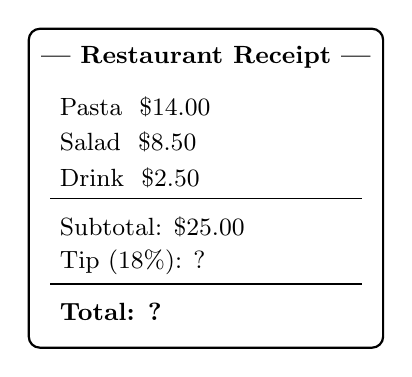
\begin{tikzpicture}[scale=0.9]
  \draw[thick,rounded corners] (0,0) rectangle (5,4.5);
  \node[font=\small\bfseries] at (2.5,4.1) {--- Restaurant Receipt ---};
  \node[anchor=west,font=\small] at (0.3,3.4) {Pasta \dotfill\ $\$14.00$};
  \node[anchor=west,font=\small] at (0.3,2.9) {Salad \dotfill\ $\$8.50$};
  \node[anchor=west,font=\small] at (0.3,2.4) {Drink \dotfill\ $\$2.50$};
  \draw[thin] (0.3,2.1) -- (4.7,2.1);
  \node[anchor=west,font=\small] at (0.3,1.7) {Subtotal: $\$25.00$};
  \node[anchor=west,font=\small] at (0.3,1.2) {Tip (18\%): ?};
  \draw[thick] (0.3,0.9) -- (4.7,0.9);
  \node[anchor=west,font=\small\bfseries] at (0.3,0.5) {Total: ?};
\end{tikzpicture}
\end{center}
\end{questionText}
\correctAnswer{Tip $= \$4.50$; Total $= \$29.50$}
\explanation{Tip: $25.00 \times 0.18 = \$4.50$. Total: $25.00 + 4.50 = \$29.50$.}
\end{practiceQuestion}

\begin{practiceQuestion}{2-5-q30}{gsa}
\begin{questionText}
The bar graph shows the monthly sales for a salesperson over $4$ months. She earns $6\%$ commission. What is her total commission for all $4$ months?

\begin{center}
\begin{tikzpicture}[scale=0.5]
  \draw[thick,->] (0,0) -- (0,7) node[above]{\small Sales (\$)};
  \draw[thick,->] (0,0) -- (9.5,0);
  \fill[funBlue!60] (0.5,0) rectangle (1.5,4);
  \fill[funBlue!60] (2.5,0) rectangle (3.5,5);
  \fill[funBlue!60] (4.5,0) rectangle (5.5,3);
  \fill[funBlue!60] (6.5,0) rectangle (7.5,6);
  \node[below,font=\small] at (1,0) {Jan};
  \node[below,font=\small] at (3,0) {Feb};
  \node[below,font=\small] at (5,0) {Mar};
  \node[below,font=\small] at (7,0) {Apr};
  \foreach \y/\lab in {2/4000,4/8000,6/12000} {
    \draw (-0.1,\y) -- (0.1,\y) node[left,font=\small,xshift=-2pt] {\lab};
  }
  \node[above,font=\small] at (1,4) {$8{,}000$};
  \node[above,font=\small] at (3,5) {$10{,}000$};
  \node[above,font=\small] at (5,3) {$6{,}000$};
  \node[above,font=\small] at (7,6) {$12{,}000$};
\end{tikzpicture}
\end{center}
\end{questionText}
\correctAnswer{$\$2{,}160$}
\explanation{Total sales: $8{,}000 + 10{,}000 + 6{,}000 + 12{,}000 = \$36{,}000$. Commission: $36{,}000 \times 0.06 = \$2{,}160$.}
\end{practiceQuestion}
